\chapter{Confucianism: Ethics, Family and the State}

\section{Context: the Warring States and the ``Hundred Schools''}

Confucius lived at the end of the Spring and Autumn period, when the Zhou kings had lost
real power and regional lords fought one another. The question every thinker of the
period asked was: \emph{how can order be restored?} The answers of the ``Hundred Schools
of Thought'' (\zht{諸子百家}) shaped Chinese political culture permanently.

\begin{center}
\begin{tabular}{lll}
\toprule
School & Key figures & Answer to disorder \\
\midrule
Confucians (\zht{儒家}, Rújiā) & Confucius, Mencius, Xunzi & moral cultivation, ritual, virtuous rulers \\
Daoists (\zht{道家}, Dàojiā) & Laozi, Zhuangzi & return to simplicity, non-action \\
Mohists (\zht{墨家}, Mòjiā) & Mozi & impartial care, frugality, anti-war \\
Legalists (\zht{法家}, Fǎjiā) & Shang Yang, Han Feizi & strict laws, rewards and punishments \\
\bottomrule
\end{tabular}
\end{center}

\section{Confucius (551--479 BCE)}

Kong Qiu (\zht{孔丘}), honoured as Kongzi or Kong Fuzi (``Master Kong'', Latinized by
Jesuits as ``Confucius''), was a minor official and teacher from the state of Lu. He saw
himself as a \emph{transmitter, not a creator}: he wanted to restore the ideals of the
early Zhou. His sayings were collected by disciples in the \emph{Analects}
(\zht{論語}, Lúnyǔ).

\subsection{Key concepts}

\begin{center}
\begin{tabular}{llp{8cm}}
\toprule
Term & Pinyin & Meaning \\
\midrule
\zht{仁} & rén & humaneness, benevolence; the highest virtue, care for others \\
\zht{禮} & lǐ & ritual propriety: ceremonies, etiquette, the proper forms of conduct \\
\zht{孝} & xiào & filial piety: devotion to parents and ancestors \\
\zht{義} & yì & righteousness: doing what is right rather than what is profitable \\
\zht{君子} & jūnzǐ & ``noble person'', the morally cultivated person (originally ``son of a lord'') \\
\zht{德} & dé & virtue, moral power that attracts others \\
\zht{正名} & zhèngmíng & rectification of names: roles must match reality \\
\bottomrule
\end{tabular}
\end{center}

\begin{definition}[Junzi]
Confucius transformed \emph{junzi} from a term of birth (aristocrat) into a term of
achievement (a person of cultivated character). In principle anyone could become a
junzi through study and self-cultivation. This idea later justified the examination
system.
\end{definition}

\begin{example}[Rule by virtue, not by law]
A famous paraphrase from the \emph{Analects}: if you lead people with regulations and
keep them in line with punishments, they will avoid trouble but have no sense of shame;
lead them with virtue and keep them in line with ritual, and they will have a sense of
shame and will reform themselves. This is the central contrast with Legalism.
\end{example}

\subsection{Rectification of names}

When asked what he would do first if given government, Confucius said he would
``rectify names'': let the ruler be a ruler, the minister a minister, the father a father,
the son a son. Disorder begins when people do not act according to their roles.

\section{The Five Relationships}

The five cardinal relationships (\zht{五倫}, wǔlún) were systematized after Confucius
(Mencius lists them). Each is reciprocal but hierarchical: the senior party owes
benevolence and guidance, the junior owes loyalty and obedience.

\begin{center}
\begin{tikzpicture}[
    rel/.style={draw, thick, rounded corners, minimum width=2.4cm, minimum height=0.8cm, font=\small, align=center},
    lab/.style={font=\scriptsize, align=center}]
  \foreach \i/\sen/\jun/\virt/\c in {
      0/Ruler/Subject/righteousness \zht{義}/red,
      1/Father/Son/affection \zht{親}/orange,
      2/Husband/Wife/distinction \zht{別}/yellow,
      3/Elder brother/Younger brother/precedence \zht{序}/green,
      4/Friend/Friend/trust \zht{信}/blue} {
    \node[rel, fill=\c!15] (s\i) at (\i*3.1,1.6) {\sen};
    \node[rel, fill=\c!8] (j\i) at (\i*3.1,0) {\jun};
    \draw[->, thick] (s\i) -- (j\i) node[midway, right, font=\scriptsize] {};
    \node[lab] at (\i*3.1,-0.85) {\virt};
  }
  \draw[<->, thick, blue] (s4) -- (j4);
  \node[font=\scriptsize, anchor=east] at (-1.3,1.6) {senior};
  \node[font=\scriptsize, anchor=east] at (-1.3,0) {junior};
\end{tikzpicture}
\end{center}

\begin{important}[Exam point: four of five are hierarchical]
Only friendship is between equals. Three of the five are family relationships, and the
ruler--subject relationship is modelled on father--son. The family is the template for the
state: a good son will be a loyal subject. This is why filial piety is the root virtue.
\end{important}

\section{Filial piety}

Filial piety (\zht{孝}, \emph{xiào}; Japanese \emph{kō}, Korean \emph{hyo} \ko{효})
meant obeying parents while alive, burying them properly, mourning them (traditionally
three years for a parent), and continuing ancestral sacrifices, which requires producing a
male heir. The \emph{Classic of Filial Piety} (\zht{孝經}) and the popular
\emph{Twenty-Four Paragons of Filial Piety} (Yuan dynasty) spread these ideals widely,
including stories of extreme self-sacrifice that modern readers find disturbing.

\begin{aside}
In class discussion several students related filial piety to their own families (for
example, the expectation of supporting parents financially, or the importance of
ancestral rites at Chuseok or Qingming). The professor's point: these are living
practices, but they are also \emph{reinvented} in each generation, not simply inherited.
\end{aside}

\section{Mencius and Xunzi}

\subsection{Mencius (c.\ 372--289 BCE)}

Mengzi (\zht{孟子}) argued that \textbf{human nature is good}. Everyone has ``four
sprouts'' (\zht{四端}) of virtue:

\begin{center}
\begin{tabular}{lll}
\toprule
Sprout (feeling) & Grows into & \\
\midrule
compassion & humaneness & \zht{仁} \\
shame & righteousness & \zht{義} \\
deference & propriety & \zht{禮} \\
sense of right and wrong & wisdom & \zht{智} \\
\bottomrule
\end{tabular}
\end{center}

His famous illustration: anyone who suddenly sees a child about to fall into a well feels
alarm and compassion, not to gain favour with the parents but spontaneously. Moral
education \emph{cultivates} these sprouts, as a farmer tends seedlings (and must not pull
on them to make them grow faster).

Mencius also developed the political side of the \textbf{Mandate of Heaven}
(\zht{天命}, tiānmìng): Heaven grants the right to rule to a virtuous ruler; a ruler who
oppresses the people loses it, and the people may rightfully overthrow him. ``Heaven sees
as the people see.''

\subsection{Xunzi (c.\ 310--235 BCE)}

Xunzi (\zht{荀子}) argued the opposite: \textbf{human nature is bad} (selfish), and
goodness is the result of deliberate effort, teachers and ritual, as a warped board is
straightened by steaming and pressing. Two of his students (Han Feizi and Li Si) became
leading Legalists.

\begin{center}
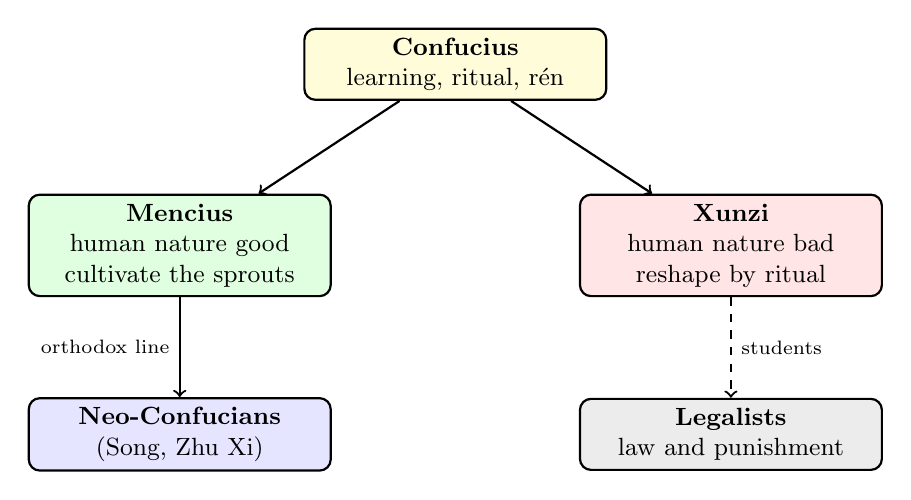
\begin{tikzpicture}[box/.style={draw, thick, rounded corners, align=center, font=\small, text width=3.6cm}]
  \node[box, fill=green!12] (m) at (-3.5,0) {\textbf{Mencius}\\human nature good\\cultivate the sprouts};
  \node[box, fill=red!10] (x) at (3.5,0) {\textbf{Xunzi}\\human nature bad\\reshape by ritual};
  \node[box, fill=yellow!15] (c) at (0,2.3) {\textbf{Confucius}\\learning, ritual, rén};
  \node[box, fill=gray!15] (l) at (3.5,-2.4) {\textbf{Legalists}\\law and punishment};
  \node[box, fill=blue!10] (n) at (-3.5,-2.4) {\textbf{Neo-Confucians}\\(Song, Zhu Xi)};
  \draw[->, thick] (c) -- (m);
  \draw[->, thick] (c) -- (x);
  \draw[->, thick, dashed] (x) -- node[right, font=\scriptsize] {students} (l);
  \draw[->, thick] (m) -- node[left, font=\scriptsize] {orthodox line} (n);
\end{tikzpicture}
\end{center}

\section{From philosophy to state orthodoxy}

\begin{enumerate}
  \item \textbf{Qin} (221--206 BCE) ruled by Legalist principles; tradition says it burned
        books and buried scholars.
  \item \textbf{Han} (206 BCE--220 CE): Emperor Wu (r.\ 141--87 BCE) made Confucianism the
        state ideology, established the Imperial Academy and recruited officials versed in
        the classics. In practice Han government was ``Confucian on the outside, Legalist on
        the inside''.
  \item \textbf{Sui--Tang}: civil service examinations begin (605 CE).
  \item \textbf{Song} (960--1279): examinations become the main route to office;
        Neo-Confucianism develops.
  \item \textbf{Ming--Qing}: Zhu Xi's commentaries on the \emph{Four Books} become the
        required curriculum (from 1313 to 1905).
\end{enumerate}

\subsection{The examination system}

\begin{center}
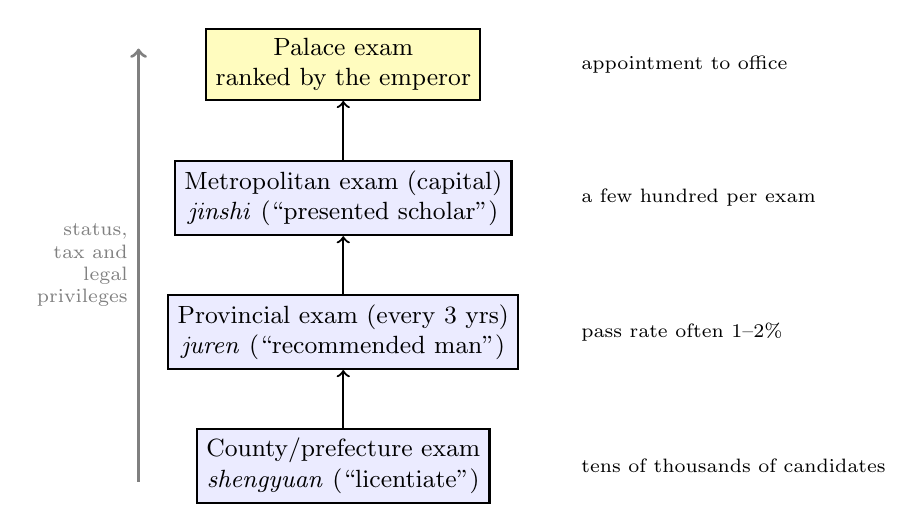
\begin{tikzpicture}[st/.style={draw, thick, fill=blue!8, align=center, font=\small,
                     minimum width=3.2cm, minimum height=0.8cm}]
  \node[st] (a) at (0,0) {County/prefecture exam\\\emph{shengyuan} (``licentiate'')};
  \node[st] (b) at (0,1.7) {Provincial exam (every 3 yrs)\\\emph{juren} (``recommended man'')};
  \node[st] (c) at (0,3.4) {Metropolitan exam (capital)\\\emph{jinshi} (``presented scholar'')};
  \node[st, fill=yellow!25] (d) at (0,5.1) {Palace exam\\ranked by the emperor};
  \draw[->, thick] (a) -- (b); \draw[->, thick] (b) -- (c); \draw[->, thick] (c) -- (d);
  \node[font=\scriptsize, anchor=west, align=left] at (2.9,0) {tens of thousands of candidates};
  \node[font=\scriptsize, anchor=west, align=left] at (2.9,1.7) {pass rate often 1--2\%};
  \node[font=\scriptsize, anchor=west, align=left] at (2.9,3.4) {a few hundred per exam};
  \node[font=\scriptsize, anchor=west, align=left] at (2.9,5.1) {appointment to office};
  \draw[->, very thick, gray] (-2.6,-0.2) -- (-2.6,5.3) node[midway, left, font=\scriptsize, align=right] {status,\\tax and\\legal\\privileges};
\end{tikzpicture}
\end{center}

\begin{itemize}
  \item Candidates memorized the Four Books (\emph{Analects}, \emph{Mencius},
        \emph{Great Learning}, \emph{Doctrine of the Mean}) and the Five Classics, and wrote
        highly formal ``eight-legged essays''.
  \item In principle open to almost all males; in practice favoured families who could
        afford years of tutoring. Still, it gave the system legitimacy and some mobility.
  \item It created the \emph{scholar-official} (literati, gentry) class that ran China.
\end{itemize}

\section{Confucianism beyond China}

\begin{center}
\begin{tabular}{lp{11cm}}
\toprule
Korea & Most thoroughly Confucianized. Goryeo held exams from 958; Joseon (1392--1910) made
Zhu Xi Neo-Confucianism the state orthodoxy, reshaped family law (patrilineal descent,
ancestor rites, eldest-son inheritance) and created the \emph{yangban} elite. \\
Japan & Confucian ideas arrived early (Prince Shōtoku's ``Seventeen Article
Constitution'', 604) but exams never took root; office remained hereditary. Neo-Confucianism
became influential in the Tokugawa period, adapted to a samurai society where
\emph{loyalty to one's lord} often outranked filial piety. \\
Vietnam & Exams from 1075 to 1919, the last in the region to abolish them. \\
\bottomrule
\end{tabular}
\end{center}

\begin{important}[Is Confucianism a religion?]
Debated. It has no creator god or church, but it has rituals (ancestor veneration, state
sacrifices at temples to Confucius) and a sense of a moral cosmos (Heaven). Most scholars
describe it as a tradition of ethical and political thought with religious dimensions.
In exams, give both sides.
\end{important}

\section{Critiques}

\begin{itemize}
  \item \textbf{Gender}: the ``three obediences'' (a woman obeys father, then husband,
        then son) and the ideal of chaste widowhood constrained women severely. Footbinding
        was \emph{not} a Confucian teaching, but it was justified in Confucian terms.
  \item \textbf{May Fourth Movement} (1919): Chinese reformers attacked ``the Confucian
        shop'' as the cause of China's weakness.
  \item \textbf{``Asian values''} (1990s): leaders such as Lee Kuan Yew claimed Confucian
        values explained East Asian economic success. Critics noted that the same
        tradition had been blamed for backwardness a few decades earlier.
\end{itemize}

\section*{Summary}
\begin{itemize}
  \item Confucius: moral cultivation, ritual, humaneness and filial piety as the basis of
        social and political order; the junzi is made, not born.
  \item Five relationships: hierarchical and reciprocal, modelled on the family.
  \item Mencius (nature good, Mandate of Heaven, right to rebel) vs.\ Xunzi (nature bad,
        ritual reshapes).
  \item Han made Confucianism state ideology; the examination system (605--1905) produced
        the scholar-official class.
  \item Korea adopted Confucian institutions most thoroughly; Japan adapted them to a
        hereditary warrior society.
\end{itemize}
